\documentclass[a4paper]{article}
\usepackage{geometry}
\usepackage{graphicx}
\usepackage{natbib}
\usepackage{amsmath}
\usepackage{amssymb}
\usepackage{amsthm}
\usepackage{paralist}
\usepackage{epstopdf}
\usepackage{tabularx}
\usepackage{longtable}
\usepackage{multirow}
\usepackage{multicol}
\usepackage[hidelinks]{hyperref}
\usepackage{fancyvrb}
\usepackage{algorithm}
\usepackage{algorithmic}
\usepackage{float}
\usepackage{paralist}
\usepackage[svgname]{xcolor}
\usepackage{enumerate}
\usepackage{array}
\usepackage{times}
\usepackage{url}
\usepackage{fancyhdr}
\usepackage{comment}
\usepackage{environ}
\usepackage{times}
\usepackage{textcomp}
\usepackage{caption}
\usepackage{color}
\usepackage{xcolor}

\urlstyle{rm}

\setlength\parindent{0pt} % Removes all indentation from paragraphs
\theoremstyle{definition}
\newtheorem{definition}{Definition}[]
\newtheorem{conjecture}{Conjecture}[]
\newtheorem{example}{Example}[]
\newtheorem{theorem}{Theorem}[]
\newtheorem{lemma}{Lemma}
\newtheorem{proposition}{Proposition}
\newtheorem{corollary}{Corollary}

\floatname{algorithm}{Procedure}
\renewcommand{\algorithmicrequire}{\textbf{Input:}}
\renewcommand{\algorithmicensure}{\textbf{Output:}}
\newcommand{\abs}[1]{\lvert#1\rvert}
\newcommand{\norm}[1]{\lVert#1\rVert}
\newcommand{\RR}{\mathbb{R}}
\newcommand{\CC}{\mathbb{C}}
\newcommand{\Nat}{\mathbb{N}}
\newcommand{\br}[1]{\{#1\}}
\DeclareMathOperator*{\argmin}{arg\,min}
\DeclareMathOperator*{\argmax}{arg\,max}
\renewcommand{\qedsymbol}{$\blacksquare$}

\definecolor{dkgreen}{rgb}{0,0.6,0}
\definecolor{gray}{rgb}{0.5,0.5,0.5}
\definecolor{mauve}{rgb}{0.58,0,0.82}

\newcommand{\Var}{\mathrm{Var}}
\newcommand{\Cov}{\mathrm{Cov}}

\newcommand{\vc}[1]{\boldsymbol{#1}}
\newcommand{\xv}{\vc{x}}
\newcommand{\Sigmav}{\vc{\Sigma}}
\newcommand{\alphav}{\vc{\alpha}}
\newcommand{\muv}{\vc{\mu}}

\newcommand{\red}[1]{\textcolor{red}{#1}}

\def\x{\mathbf x}
\def\y{\mathbf y}
\def\w{\mathbf w}
\def\v{\mathbf v}
\def\E{\mathbb E}
\def\V{\mathbb V}

% TO SHOW SOLUTIONS, include following (else comment out):
\newenvironment{soln}{
    \leavevmode\color{blue}\ignorespaces
}{}


\hypersetup{
%    colorlinks,
    linkcolor={red!50!black},
    citecolor={blue!50!black},
    urlcolor={blue!80!black}
}

\geometry{
  top=1in,            % <-- you want to adjust this
  inner=1in,
  outer=1in,
  bottom=1in,
  headheight=3em,       % <-- and this
  headsep=2em,          % <-- and this
  footskip=3em,
}


\pagestyle{fancyplain}
\lhead{\fancyplain{}{Homework 2}}
\rhead{\fancyplain{}{CS 760 Machine Learning}}
\cfoot{\thepage}

\title{\textsc{Homework 2}} % Title

%%% NOTE:  Replace 'NAME HERE' etc., and delete any "\red{}" wrappers (so it won't show up as red)

\author{
Martino Boggs \\
ID: 907 810 3539
} 

\date{}

\begin{document}

\maketitle 


\textbf{Instructions:} 
Use this latex file as a template to develop your homework. Submit your homework on time as a single pdf file to Canvas. Please wrap your code and upload to a public GitHub repo, then attach the link below the instructions so that we can access it. You can choose any programming language (i.e. python, R, or MATLAB), as long as you implement the algorithm from scratch (e.g. do not use sklearn on questions 1 to 7 in section 2). Please check Piazza for updates about the homework.

\section{A Simplified Decision Tree}
You are to implement a decision-tree learner for classification.
To simplify your work, this will not be a general purpose decision tree.  Instead, your program can assume that
\begin{itemize}
\item each item has two continuous features $\x \in \RR^2$
\item the class label is binary and encoded as $y \in \{0,1\}$
\item data files are in plaintext with one labeled item per line, separated by whitespace:
$$x_{11} \quad x_{12} \quad y_1$$
$$...$$
$$x_{n1} \quad x_{n2} \quad y_n$$
\end{itemize}

Your program should implement a decision tree learner according to the following guidelines:
\begin{itemize}
\item Candidate splits $(j,c)$ for numeric features should use a threshold $c$ in feature dimension $j$ in the form of $x_{\cdot j}\ge c$.
\item $c$ should be on values of that dimension present in the training data; i.e. the threshold is on training points, not in between training points. You may enumerate all features, and for each feature, use all possible values for that dimension.
\item You may skip those candidate splits with zero split information (i.e. the entropy of the split), and continue the enumeration.
\item The left branch of such a split is the ``then'' branch, and the right branch is ``else''.
\item Splits should be chosen using information gain ratio. If there is a tie you may break it arbitrarily.
\item The stopping criteria (for making a node into a leaf) are that 
	\begin{itemize}
	\item the node is empty, or
	\item all splits have zero gain ratio (if the entropy of the split is non-zero), or
	\item the entropy of any candidates split is zero
	\end{itemize}
\item To simplify, whenever there is no majority class in a leaf, let it predict $y=1$.
\end{itemize}

\begin{soln} See code on GitHub: \end{soln}

\section{Questions}
\begin{enumerate}
\item (Our algorithm stops at pure labels) [10 pts] If a node is not empty but contains training items with the same label, why is it guaranteed to become a leaf?  Explain. You may assume that the feature values of these items are not all the same. \\

\begin{soln}
  If the training items have the same label $y^*$, then $Y = y^*$ is a constant random variable and thus is independent of any candidate split $S$. It follows that the empirical entropy of $Y$ and $Y|S$ is 
  $$\begin{aligned}
  H_D(Y) &= -\sum_{y \:\in\: \mathcal{Y}}\mathbb{P}(Y=y)\log_2\mathbb{P}(Y=y) = -\mathbb{P}(Y = y^*)\log_2\mathbb{P}(Y=y^*)=0 \\[1ex]
  H_D(Y|S) &= -\sum_{s\:\in\:\mathcal{S}} \sum_{y \:\in\:\mathcal{Y}} \mathbb{P}(S=s)\mathbb{P}(Y=y|S=s)\log_2\mathbb{P}(Y=y|S=s)\\[1ex]
  &=-\sum_{s\:\in\:\mathcal{S}}\mathbb{P}(S=s)\mathbb{P}(Y=y^*)\log_2\mathbb{P}(Y=y^*) = 0
  \end{aligned}$$ since $\log_2\mathbb{P}(Y=y^*)=\log_2(1)=0$. Therefore, the information gain ratio of the candidate split is zero and our algorithm creates a leaf node.
\end{soln}

\item (Our algorithm is greedy)  [10 pts] Handcraft a small training set where both classes are present but the algorithm refuses to split; instead it makes the root a leaf and stop;
Importantly, if we were to manually force a split, the algorithm will happily continue splitting the data set further and produce a deeper tree with zero training error.
You should (1) plot your training set, (2) explain why.  Hint: you don't need more than a handful of items. \\

\begin{soln}
  The algorithm will turn the root into a leaf node if all candidate splits have zero gain ratio. In this example, our training set has both classes present, but the features $x_1$ and $x_2$ are non-informative. That is for each observation with label $y = 1$, there is an observation labelled $y = 0$ with the same features $x_1, x_2$. The candidate splits will have zero gain ratio and the algorithm will return the prediction $y=1$.
\end{soln}

\begin{figure}[htbp]
  \centerline{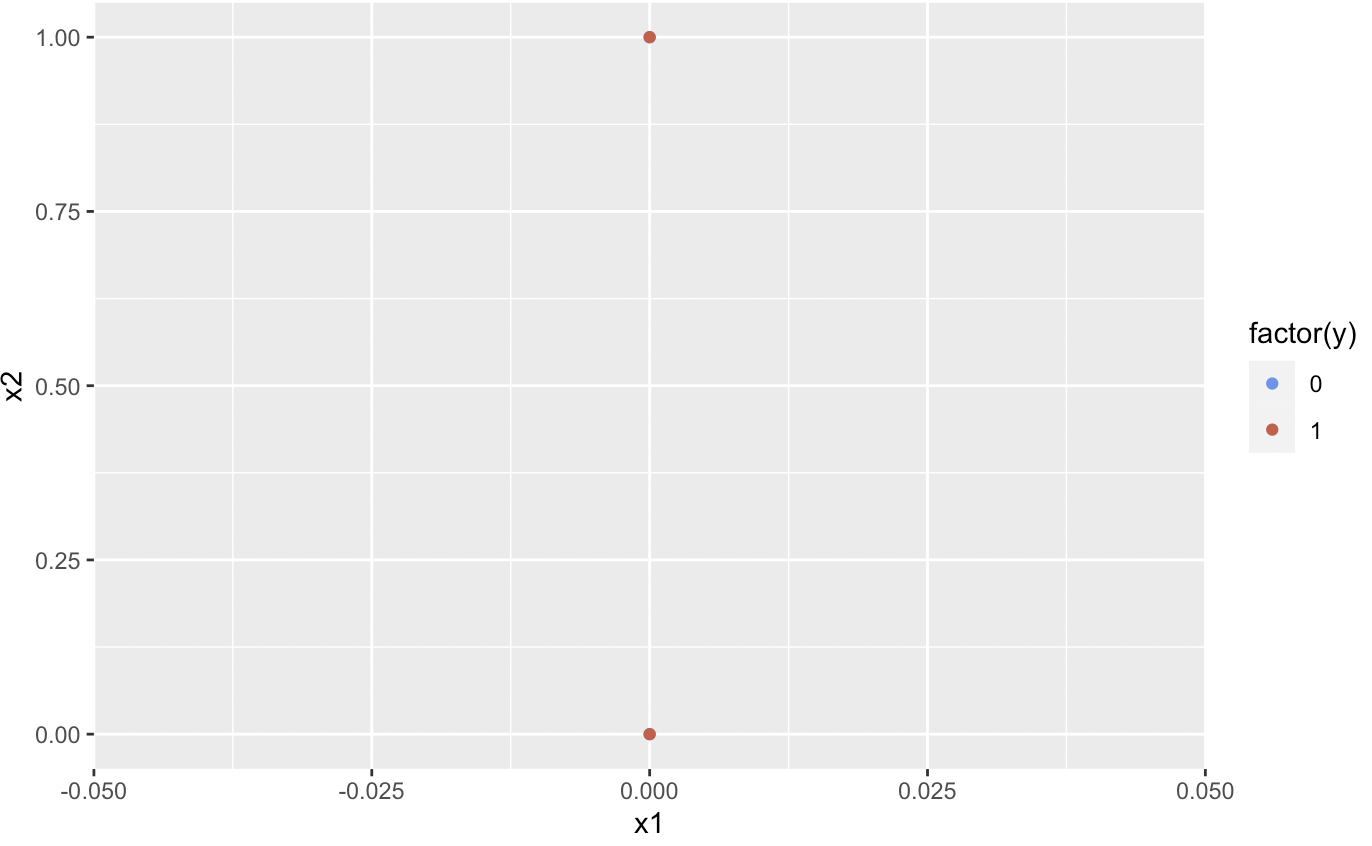
\includegraphics[scale=.5]{Q2.png}}
\end{figure}

\pagebreak

\item (Information gain ratio exercise)  [10 pts] Use the training set Druns.txt.  For the root node, list all candidate cuts and their information gain ratio. If the entropy of the candidate split is zero, please list its mutual information (i.e. information gain). Hint: to get $\log_2(x)$ when your programming language may be using a different base, use \verb|log(x)/log(2)|. Also, please follow the split rule in the first section. \\

\begin{figure}[htbp]
  \centerline{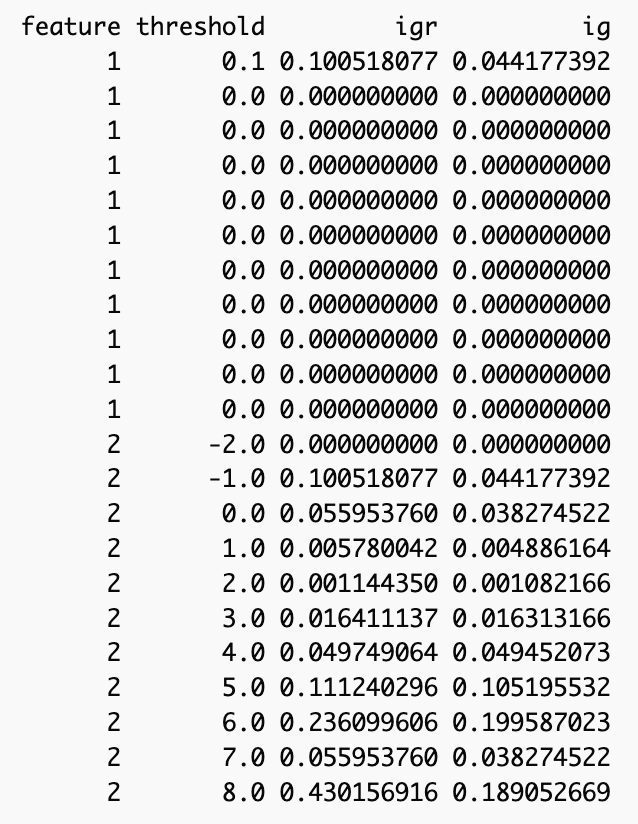
\includegraphics[scale=0.5]{Q3.png}}
\end{figure}

\item (The king of interpretability)  [10 pts] Decision tree is not the most accurate classifier in general.  However, it persists.  This is largely due to its rumored interpretability: a data scientist can easily explain a tree to a non-data scientist.  Build a tree from D3leaves.txt.  Then manually convert your tree to a set of logic rules.  Show the tree\footnote{When we say show the tree, we mean either the standard computer science tree view, or some crude plaintext representation of the tree -- as long as you explain the format.  When we say visualize the tree, we mean a plot in the 2D $\x$ space that shows how the tree will classify any points.} and the rules. \\

\begin{soln}
  If $x_1 \geq 10$, then predict $y=1$; otherwise, predict $y=1$ if $x_2 \geq3$ or predict $y=0$ if $x_2 < 3$.
\end{soln}

\begin{figure}[htbp]
  \centerline{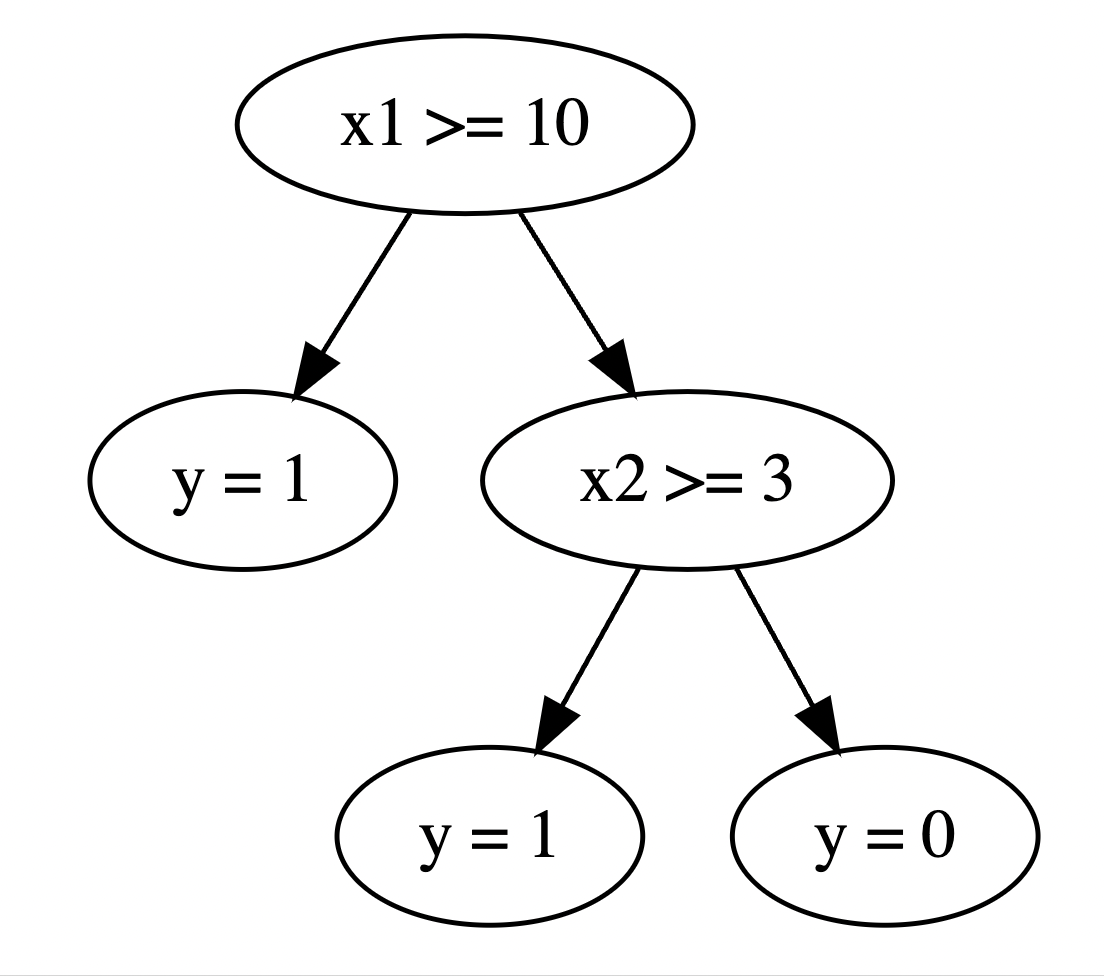
\includegraphics[scale=0.5]{Q4.png}}
\end{figure}

\pagebreak

\item (Or is it?)  [20 pts] For this question only, make sure you DO NOT VISUALIZE the data sets or plot your tree's decision boundary in the 2D $\x$ space.  If your code does that, turn it off before proceeding.  This is because you want to see your own reaction when trying to interpret a tree.  You will get points no matter what your interpretation is.
And we will ask you to visualize them in the next question anyway.
  \begin{itemize}
  
  \item Build a decision tree on D1.txt.  Show it to us in any format (e.g. could be a standard binary tree with nodes and arrows, and denote the rule at each leaf node; or as simple as plaintext output where each line represents a node with appropriate line number pointers to child nodes; whatever is convenient for you). Again, do not visualize the data set or the tree in the $\x$ input space.  In real tasks you will not be able to visualize the whole high dimensional input space anyway, so we don't want you to ``cheat'' here. \\
  
  \begin{figure}[htbp]
    \centerline{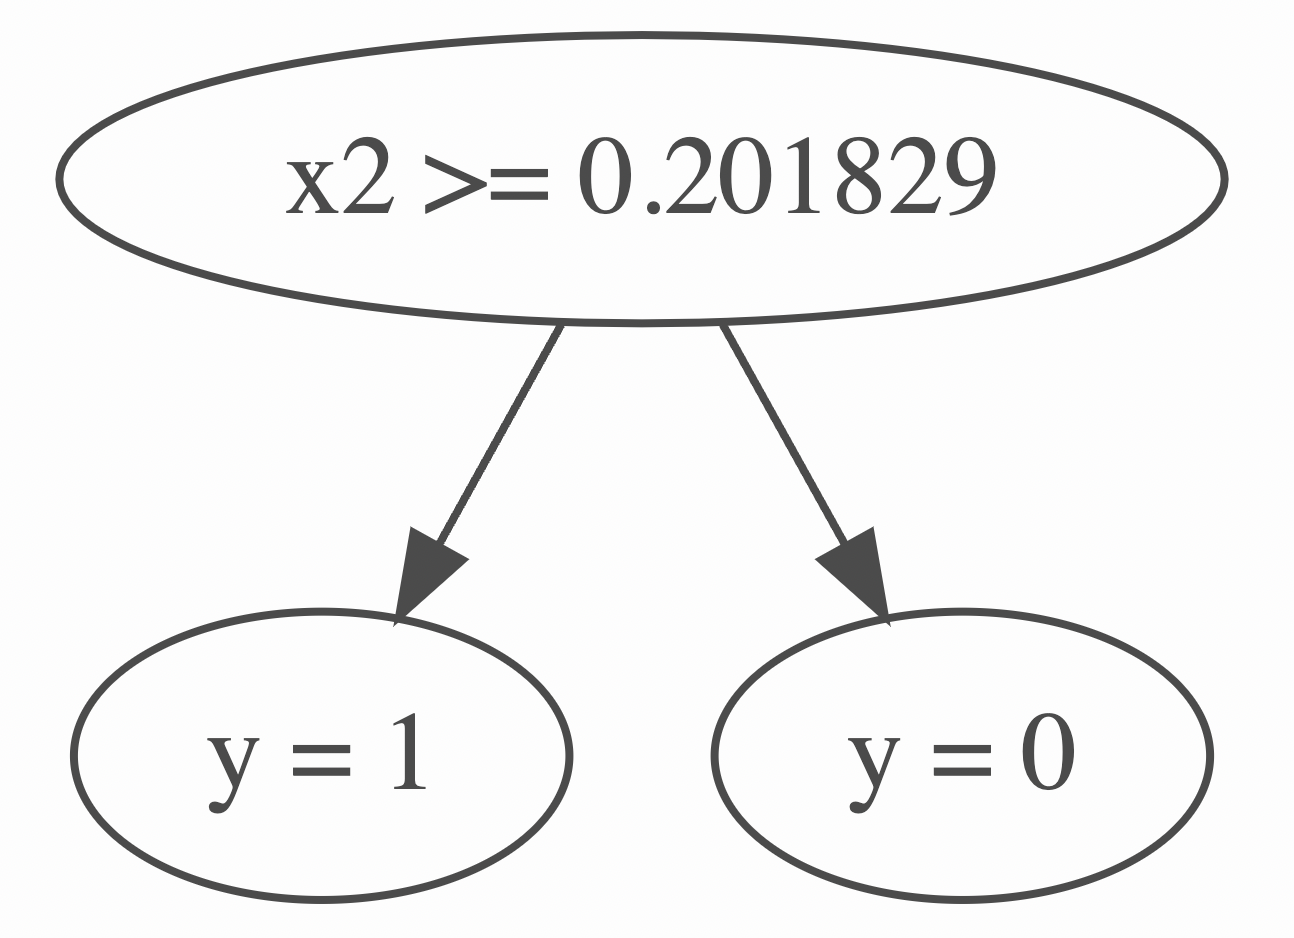
\includegraphics[scale=0.35]{Q5a.png}}
  \end{figure}

  \item Look at your tree in the above format (remember, you should not visualize the 2D dataset or your tree's decision boundary) and try to interpret the decision boundary in human understandable English. \\
  

  \begin{soln}
    For D1.txt, the decision boundary is the horizontal line $x_2 = 0.201829$. Training points in the dataset above this line are predicted to have label $y=1$, and points below this line are predicted to have label $y = 0$.
  \end{soln}

  \item Build a decision tree on D2.txt.  Show it to us. \\
  
  \begin{figure}[htbp]
    \centerline{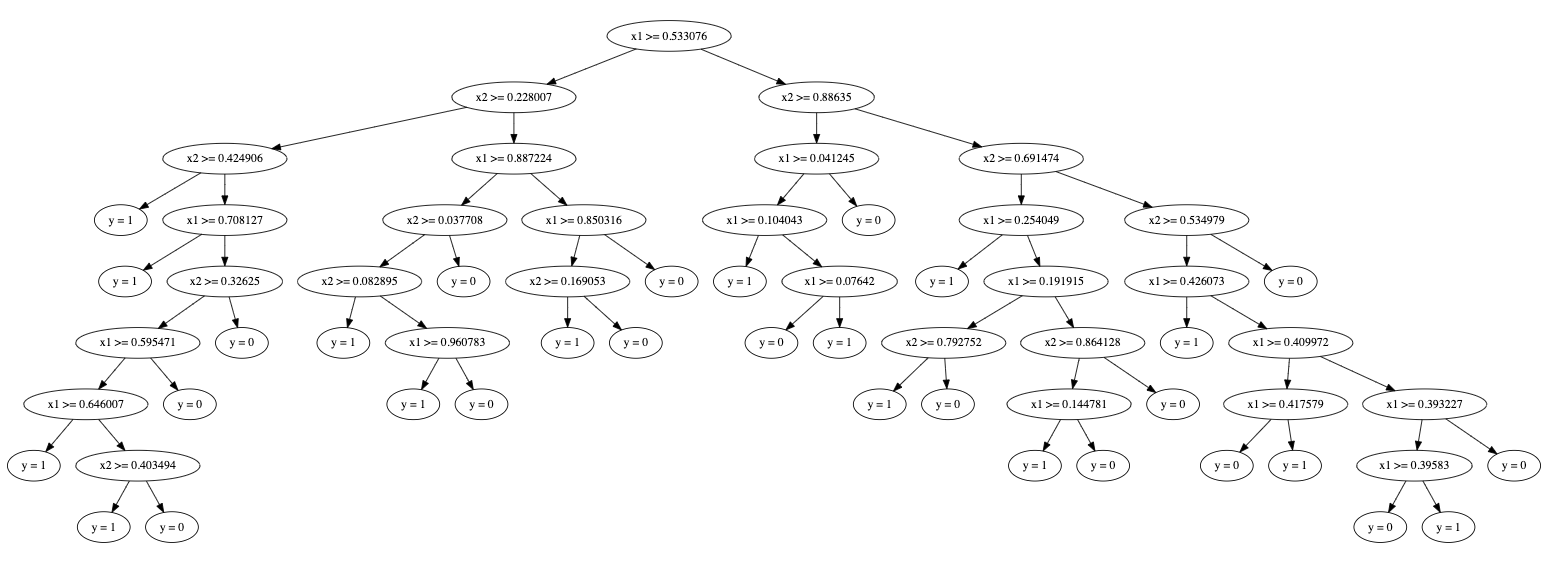
\includegraphics[scale=0.55]{Q5b.png}}
  \end{figure}
  
  \item Try to interpret your D2 decision tree. Is it easy or possible to do so without visualization? \\
  
  \begin{soln}
    The decision tree for `D2.txt` is much larger than the previous one and is more challenging to interpret without visualization. The decision boundary involves both $x_1$ and $x_2$ (i.e., not a horizontal or vertical line). Training points in this dataset seem to be predicted to have label $y=1$ if either $x_1$ or $x_2$ are sufficiently large. For example, the decision tree predicts $y = 1$ for both training points $(x_1, x_2) = (.97, .05)$ and $(x_1, x_2) = (.11, .88)$. It also predicts $y = 1$ for $(x_1, x_2) = (0.54, 0.43)$, but predicts $y = 0$ for $(x_1, x_2) = (0.53, 0.53)$. The decision boundary may be a line with a negative slope (e.g., close to $x_2=1-x_1$).
  \end{soln}

  \end{itemize}

\item (Hypothesis space)  [10 pts] For D1.txt and D2.txt, do the following separately:
  \begin{itemize}
  
  \item Produce a scatter plot of the data set.

  \item Visualize your decision tree's decision boundary (or decision region, or some other ways to clearly visualize how your decision tree will make decisions in the feature space).

  \begin{figure}[htbp]
    \centerline{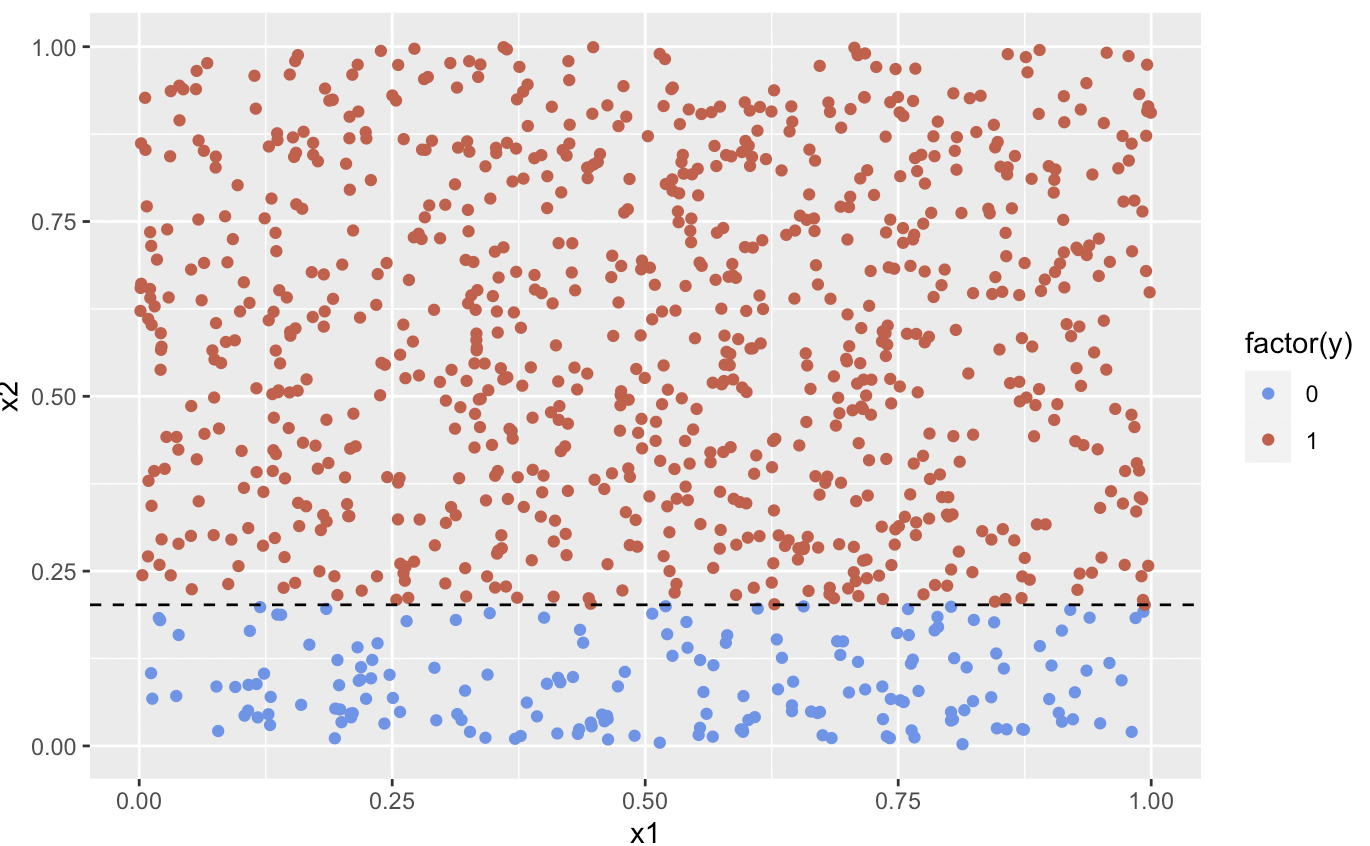
\includegraphics[scale=0.5]{Q6a.png}}
  \end{figure}

  \begin{figure}[htbp]
    \centerline{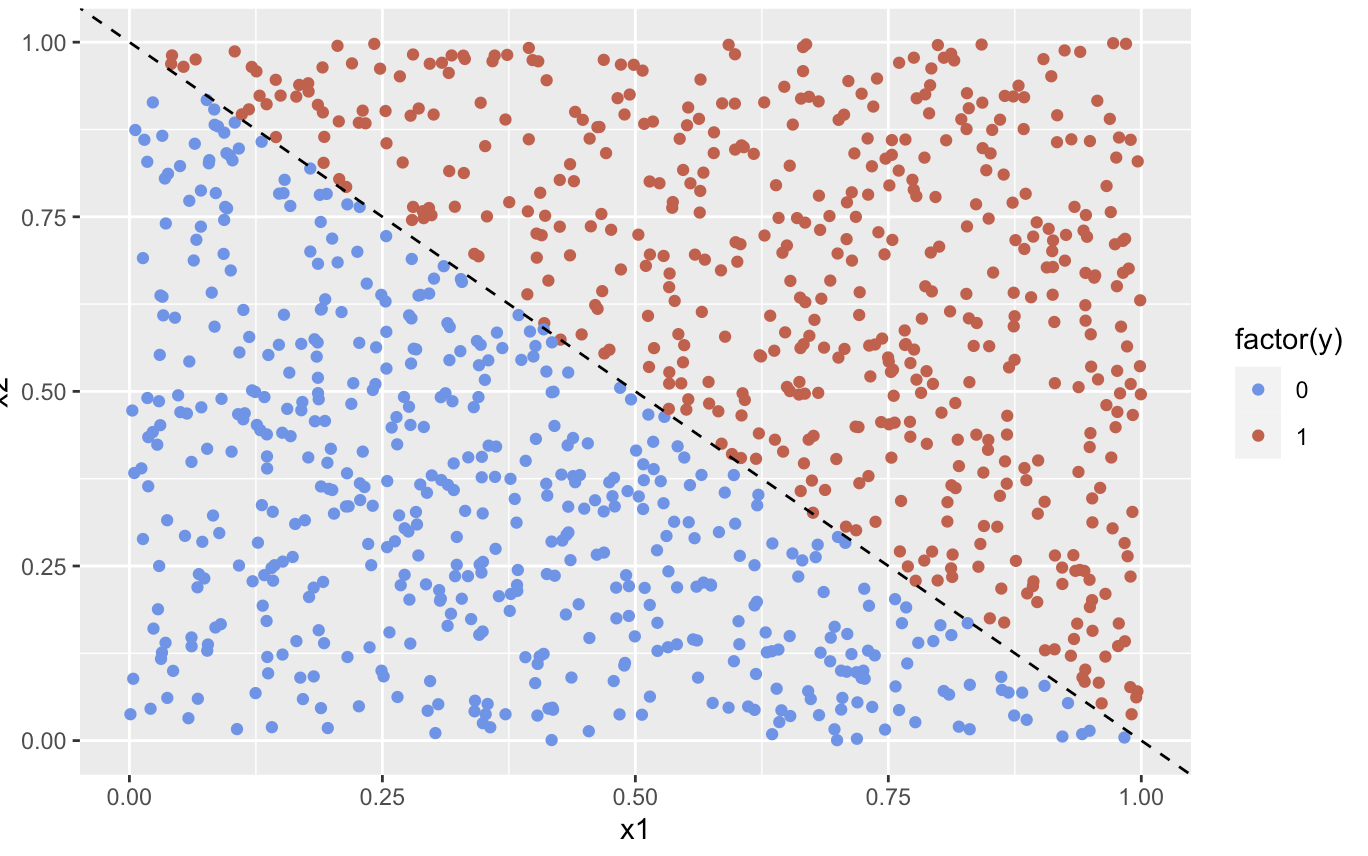
\includegraphics[scale=0.5]{Q6b.png}}
  \end{figure}


  \end{itemize}
Then discuss why the size of your decision trees on D1 and D2 differ.  Relate this to the hypothesis space of our decision tree algorithm. \\

\begin{soln}
For D1, we only need to split on the feature $x_2$ since it alone determines the label $y$. The size of the decision tree on D2 is larger since the label $y$ depends on both $x_1$ and $x_2$. The hypothesis space for our decision tree algorithm is the set of all possible decision trees using candidate splits on $x_1$ and $x_2$. Since $x_1$ provides no information gain, the hypothesis space for the decision tree on D1 is constrained than that of decision tree on D2.
\end{soln}

\pagebreak

\item (Learning curve)  [20 pts] We provide a data set Dbig.txt with 10000 labeled items.  Caution: Dbig.txt is sorted.
  \begin{itemize}
  
  \item You will randomly split Dbig.txt into a candidate training set of 8192 items and a test set (the rest).  Do this by generating a random permutation, and split at 8192.
  
  \item Generate a sequence of five nested training sets $D_{32} \subset D_{128} \subset D_{512} \subset D_{2048} \subset D_{8192}$ from the candidate training set.  The subscript $n$ in $D_n$ denotes training set size.  The easiest way is to take the first $n$ items from the (same) permutation above.  This sequence simulates the real world situation where you obtain more and more training data.
  
  \item For each $D_n$ above, train a decision tree.  Measure its test set error $err_n$.  Show three things in your answer: (1) List $n$, number of nodes in that tree, $err_n$. (2) Plot $n$ vs. $err_n$.  This is known as a learning curve (a single plot). (3) Visualize your decision trees' decision boundary (five plots). \\
  \end{itemize}

\begin{soln}
  Note that error is number of misclassified data points in test set (out of 1808).
\end{soln}

  \begin{figure}[htbp]
    \centerline{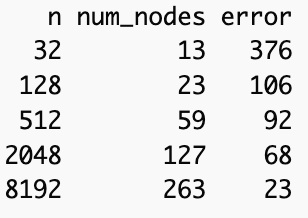
\includegraphics[scale=1]{Q7a.png}}
  \end{figure}

  \begin{figure}[htbp]
    \centerline{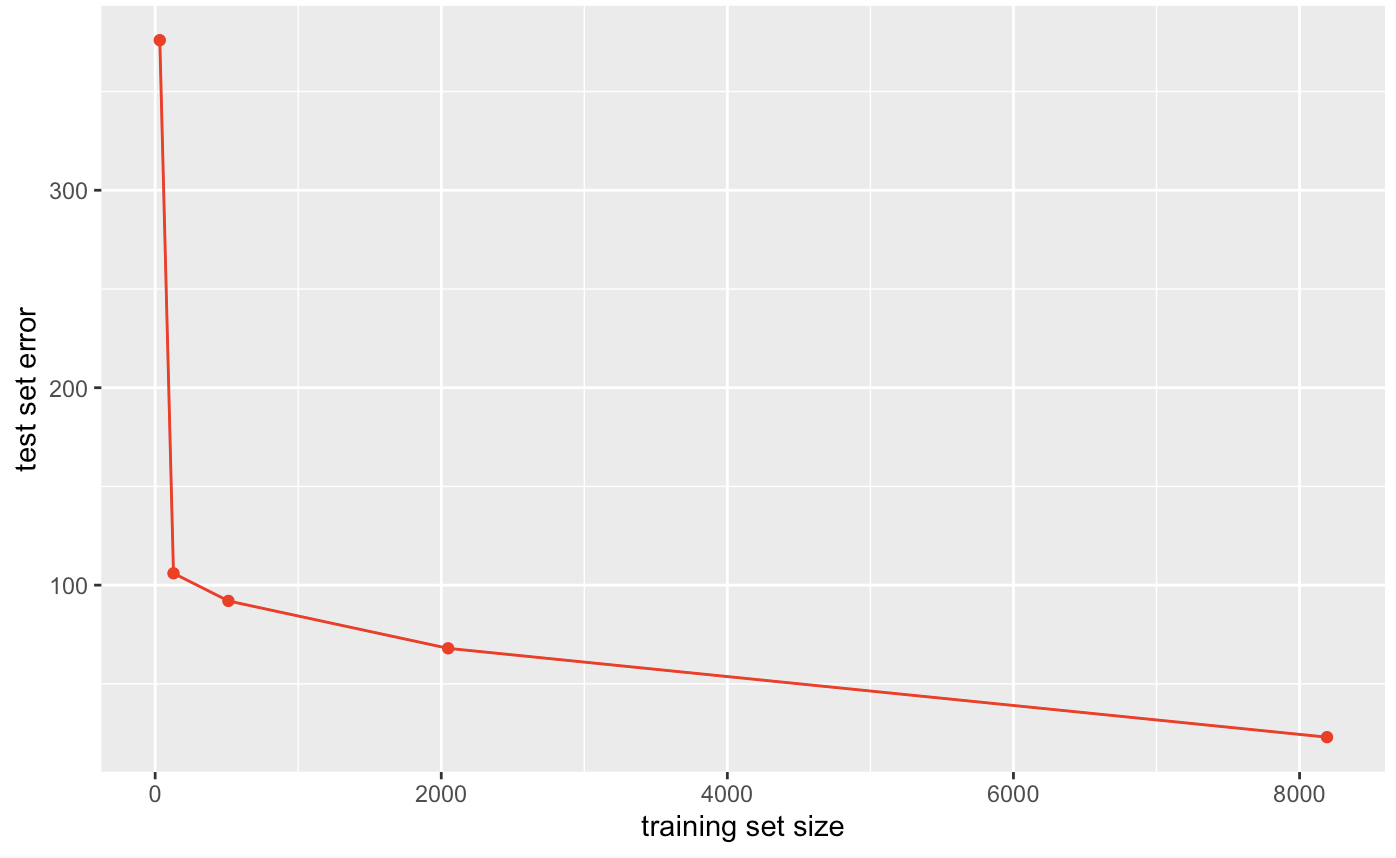
\includegraphics[scale=0.5]{Q7b.png}}
  \end{figure}

  \begin{figure}[htbp]
    \centerline{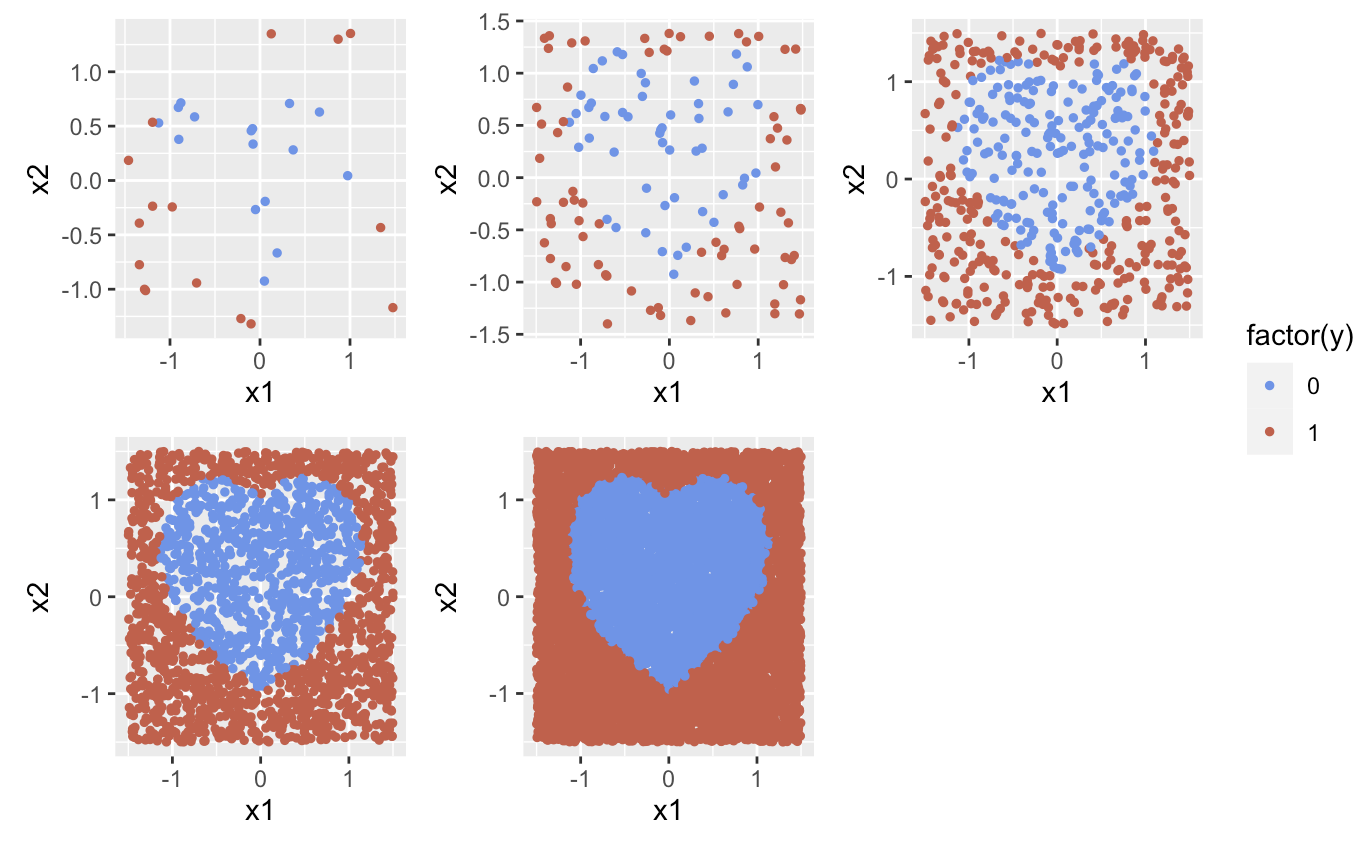
\includegraphics[scale=0.75]{Q7c.png}}
  \end{figure}
  
\end{enumerate}

\pagebreak

\section{sklearn [10 pts]}
Learn to use sklearn (\url{https://scikit-learn.org/stable/}).
Use sklearn.tree.DecisionTreeClassifier to produce trees for datasets $D_{32}, D_{128}, D_{512}, D_{2048}, D_{8192}$.  Show two things in your answer: (1) List $n$, number of nodes in that tree, $err_n$. (2) Plot $n$ vs. $err_n$. \\

\begin{soln}
  Note that error is number of misclassified data points in test set (out of 1808).
\end{soln}

\begin{figure}[htbp]
  \centerline{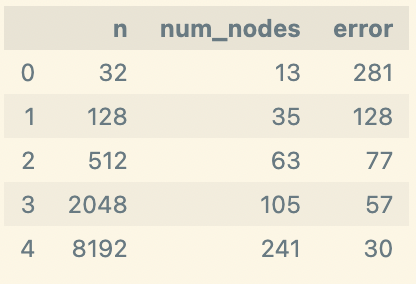
\includegraphics[scale=0.75]{sklearn.png}}
\end{figure}

\begin{figure}[htbp]
  \centerline{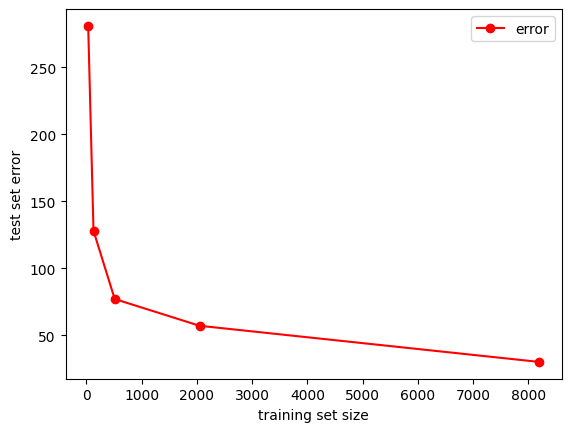
\includegraphics[scale=0.75]{learning_curve.png}}
\end{figure}

\pagebreak

\section{Lagrange Interpolation [10 pts]}
Fix some interval $[a, b]$ and sample $n = 100$ points $x$ from this interval uniformly. Use these to build a training set consisting of $n$ pairs $(x, y)$ by setting function $y = sin(x)$. \\

Build a model $f$ by using Lagrange interpolation, check more details in \url{https://en.wikipedia.org/wiki/Lagrange_polynomial} and \url{https://docs.scipy.org/doc/scipy/reference/generated/scipy.interpolate.lagrange.html}. \\

Generate a test set using the same distribution as your test set. Compute and report the resulting model’s train and test error. What do you observe?
Repeat the experiment with zero-mean Gaussian noise $\epsilon$ added to $x$. Vary the standard deviation for $\epsilon$ and report your findings. \\

\begin{soln}
  We sample $n=19$ points uniformly from $[0, 4]$ and set $y_i=\sin(x_i)$ for $i=1,\dots,19$. We fit a model using Lagrange interpolation. (Note that fitting a model with more than nineteen points using `lagrange` from the `scipy` package results in numerical errors and absurdly large MSE.) The MSEs computed on the training set and test set were 0.001 and 0.011, respectively. The model fits the sine curve fairly well (barring issues with numerical errors). \\[1ex]

  Let $x_i \sim U(0, 4)$, $y_i = \sin(x_i)$, and fit a model using Lagrange interpolation on $(x_i + \epsilon_i, y_i)$ where $\epsilon_i \sim \mathcal{N}(0, 1)$ for $i=1,\dots,19$. The MSEs computed on the training set and test set (with no Gaussian noise) were 0.056 and $1.57\times10^{8}$. The test error is much larger than the train error setting $\sigma = 1$. Since our model was fit using noisy data, it doesn't capture the true distribution of $(x_i, y_i)$. Increasing $\sigma$ by a factor of 100 seems to reduce both the train and test error, although the test error is still much larger than the train error and our model doesn't capture the sine curve we are trying to learn. Reducing $\sigma$ by a factor of 100 also tends to reduce both the train and test error (and are closer in magnitude). 
\end{soln}

\bibliographystyle{apalike}
\end{document}
